% !TEX root = $uni/master-thesis/thesis/main.tex
\documentclass[../trend-calculus.tex]{subfiles}

\begin{document}
  
  \begin{figure}
    \centering
    \begin{subfigure}{\textwidth}
      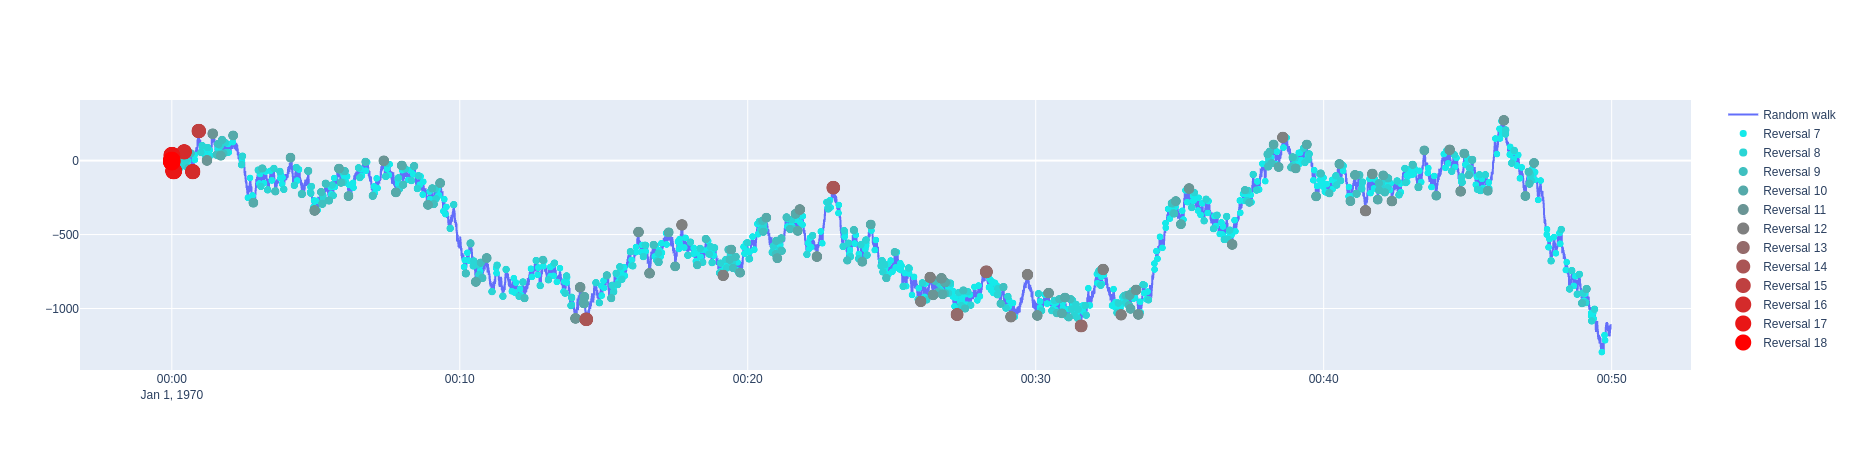
\includegraphics[width=0.98\textwidth]{graphics/trinomial-rw1.png}
      \caption{Reversals in a trinomial random walk. $|T| = 3 \cdot 10^6$.}
    \end{subfigure}
    \begin{subfigure}{\textwidth}
      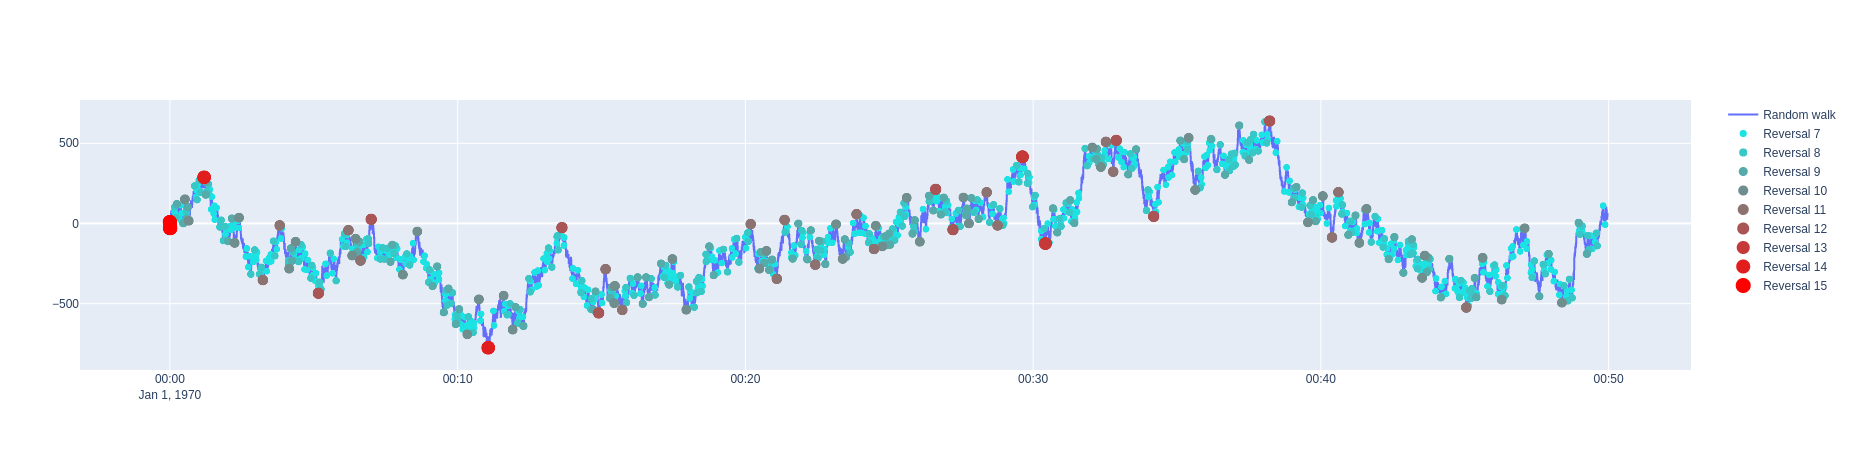
\includegraphics[width=0.98\textwidth]{graphics/trinomial-rw2.png}
      \caption{Reversals in a trinomial random walk. $|T| = 3 \cdot 10^6$.}
    \end{subfigure}
    \begin{subfigure}{\textwidth}
      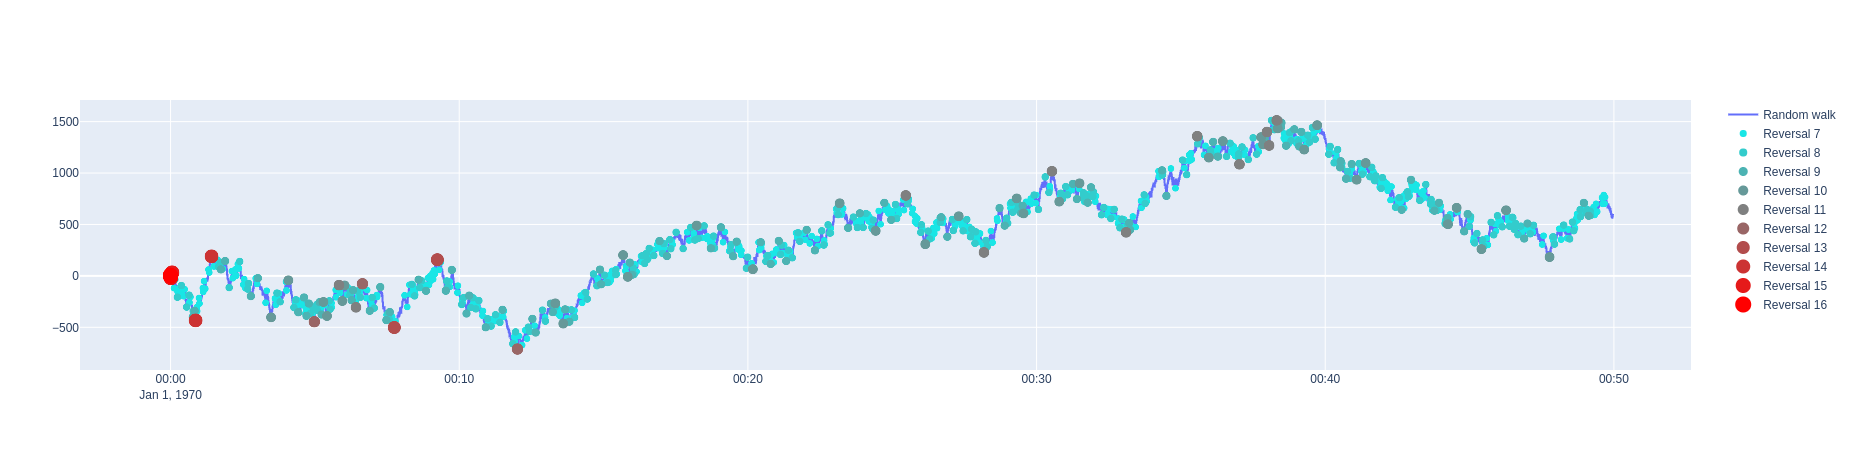
\includegraphics[width=0.98\textwidth]{graphics/trinomial-rw3.png}
      \caption{Reversals in a trinomial random walk. $|T| = 3 \cdot 10^6$.}
    \end{subfigure}
    \begin{subfigure}{\textwidth}
      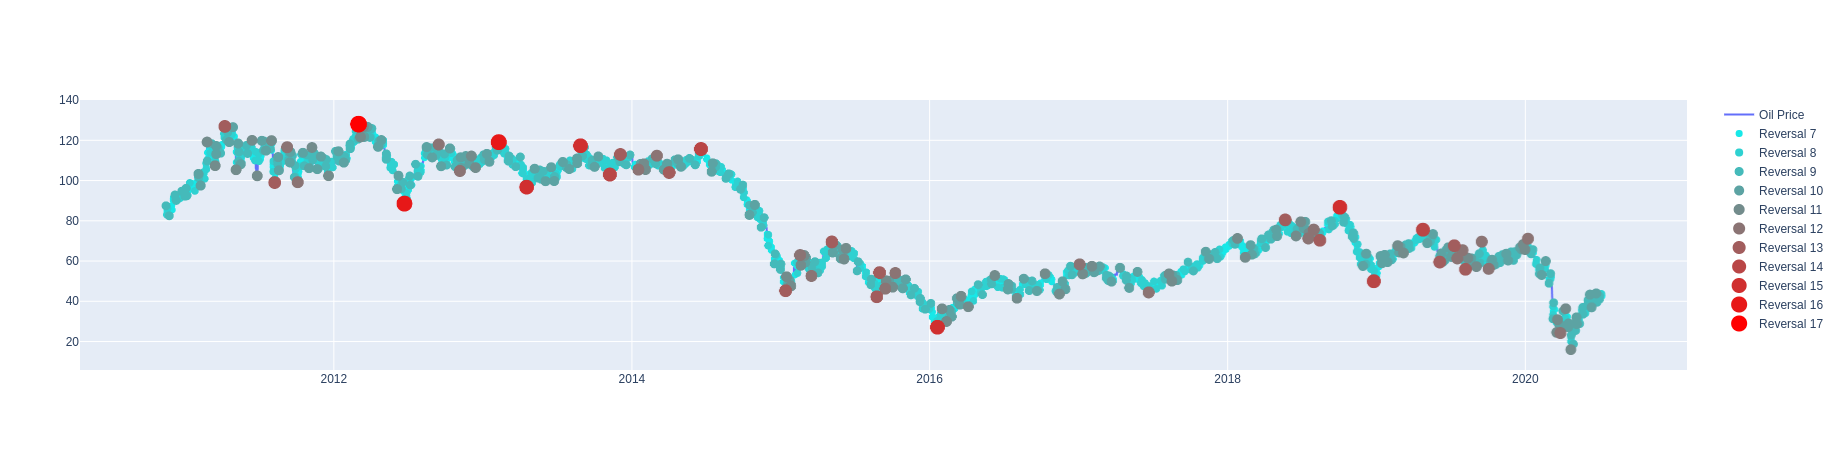
\includegraphics[width=0.98\textwidth]{graphics/tc-oil.png}
      \caption{Reversals in oil price (2010 - 2020). $|T| = 2.86 \cdot 10^6$.}
    \end{subfigure}
    \begin{subfigure}{\textwidth}
      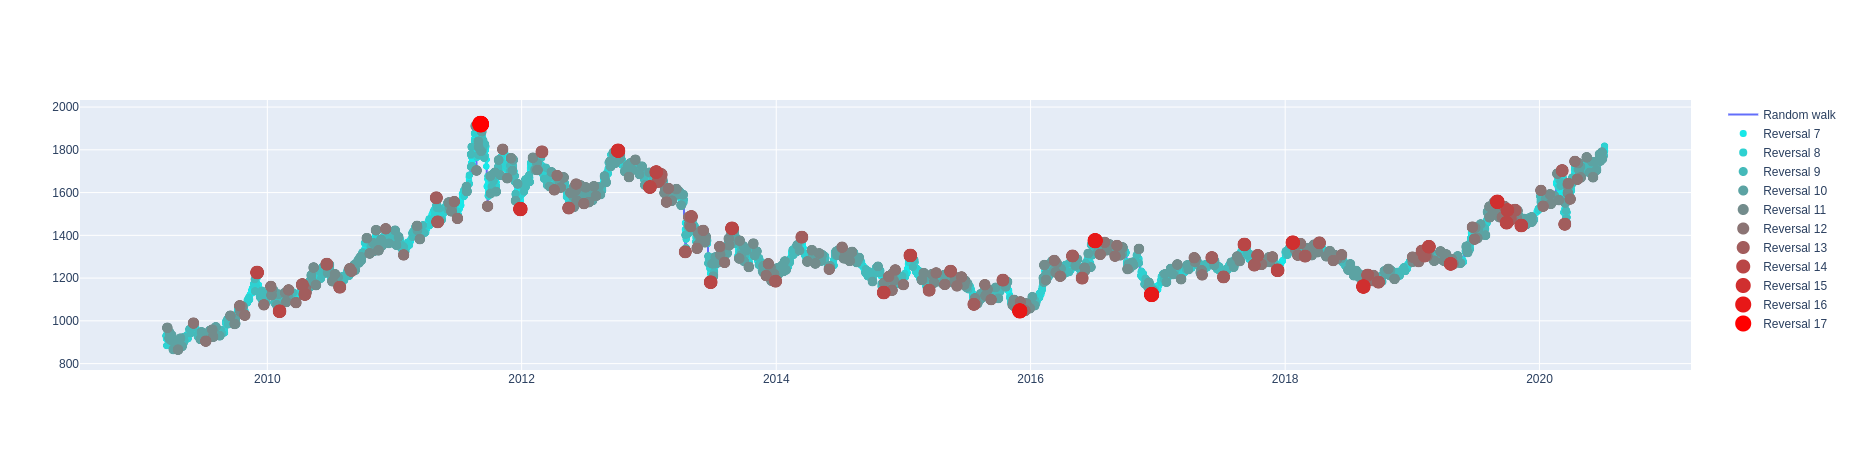
\includegraphics[width=0.98\textwidth]{graphics/tc-gold.png}
      \caption{Reversals in gold price (2010 - 2020). $|T| = 3.99 \cdot 10^6$.}
    \end{subfigure}
    \caption{Trend reversals in three realizations of trinomial random walks with uniform probabilities, as well as two real financial time series.
    The time series lengths $|T|$ are all of the same magnitude.}
    \label{fig:trendcalculus}
  \end{figure}

\end{document}